\documentclass[a4paper,oneside,english]{book}

\usepackage[sc,osf]{mathpazo}
\usepackage{units}
\usepackage{amsmath}
\usepackage{amsfonts}
\usepackage{amssymb}
\usepackage{amsthm}
\usepackage{stmaryrd}

%\makeatletter
%%%%%%%%%%%%%%%%%%%%%%%%%%%%%% Textclass specific LaTeX commands.
\numberwithin{equation}{section}
\numberwithin{figure}{section}

%\makeatother
\newcommand{\codesorc}[1]{\texttt{github.com/mathrgo/setpso/#1}}
\usepackage{babel}
\usepackage{graphicx}
\begin{document}
	\title{Experiments in Developing Discrete Particle Swarm Optimisers}
	\author{Martin Gate}
	\maketitle
	\tableofcontents\newpage
	
	\part[Algorithms]{Algorithm Description and Justification}
	\chapter{Overview and Introduction}
	\section{Setting the  Scene}
	In many cases a complex organism in nature has a goal to survive well in a changing environment it does this by actuating various limbs or change of internal perception, exploring possible outcomes or revoking memories under the control of a nervous system to get a desired outcome. The degree of effort and lack of a expected result  can be regarded as a \emph{cost} that depends on the  environment  and sequence of actions/perceptions  that it evokes. By analogy with robots, the current algorithm and computers the system can be regarded as finding  \emph{program}  fragments to give good results most of the time so that it can respond effortlessly to changes of environment. Sometimes the program gives an unexpected costly outcome and the organism must modify the program. I believe such tweaking is done by directed random choice anything else such as deductive reasoning is really part of the program. Such choice is directed in the sense that it will be biased towards cases that worked in the past. As such the  specific program-to-outcome cost is like a \emph{cost function } but with some random fluctuation since the  same program may produce different outcomes depending on unknown-to-the-system influence in the  environment. The \emph{program} in this context can be regarded in general as decoded  \emph{input} to the function that gives a cost, the input being a string of bits while the directed random choice is to be regarded as an \emph{optimiser}; by its nature the optimiser cannot see into the workings of this function otherwise it would be part of the cost function; all it has is the cost associated with the input as a string of bits and the constraint that chosen input indeed gives a working program.\footnote{ in the algorithm a cost function tries to convert an arbitrary binary string to a meaningful input and gives it back to the optimiser. }
	
	By its nature the input generated by the optimiser is discrete so the optimiser is strictly a combinatorial one, but is continuous to the extent that a small change in the string of bits \emph{often} gives a moderate change in the associated cost or a jump to an alternative working solution.\footnote{This leads to a thought that encoding should be mutable with an additional transformation by the optimiser which is independently tuned to find a better total encoding that reflects this requirement.} This is an important requirement to ensure it works properly and puts a significant burden on the design of a cost function. In a sense the optimiser both innovates and  finds solutions by flipping bits in the input string and can be quite competitive by effectively carrying out an \emph{evidence based probabilistic binary search}.   
	 
	 The rest of this book will explore the relation between function and the above optimiser type, describing algorithms to implement them and hopefully eventually apply them to interesting  cases that are models of systems that reflect real world behaviour. 
	 
	\section{Architecture}
	
	I think it helps to have a visual over view that is a cartoon of the software  so far. Figure \ref{fig:spso-overview} gives my attempt to give this. 
	
	The examples are stored in the directory \codesorc{examples} and consist of short code snippets that can be edited to change parameters. SPSO or SPO stands for Set-based Particle Swarm Optimiser loosely based on  \cite{KE-pso} , although the current algorithms have been extended to deal with combinatorial problems, include shotgun randomisation to improve convergence and deals with noisy cost functions. 
	
	The PSOkit is a tool kit that runs the chosen optimiser or cost function, generating diagnostic output in the form of \emph{Actions} where the environment is for the moment desk-top computer running the example. There are several optimisers,  cost functions and Actions which are \emph{always} referred in the toolkit by name. The user can generate new named versions as and when needed. Using names opens the door to future cost functions being able to refer additional components at run time although implementation at this moment is too restrictive. Code for the toolkit is in directory \codesorc{psokit} .
	
	The Cost Function receives a string of bits to convert into a  bundle of components referred to as a \emph{Try}, which can be a complex object containing a program. A Try is used and generated by the Cost Function, represented as a factory, which also carry out relative cost function comparisons of Try pairs, using a function call CMP(), represented by balancing scale, when required  by the optimiser. There are two types of comparison one that compares cost represented by the \$ sign and a comparison of how frequently the try gives a better cost when compared with other tries and is represented by the rosette badge, which symbolises historic success of a try that is needed to deal with noisy costing. 
	
	A Try has a wrapper that provides an interface to the optimiser; examples are given in the directory \codesorc{fun/futil}   for different cost types. The wrapper also reduces the overhead of generating a new Cost Function  and corresponding Try from scratch, such wrapped functions are given in the directory \codesorc{fun}.
	
	The optimiser is represented by a lightbulb and base; signifying that it is like an ideas generator; this is bourn out by the way in which the optimiser jumps to significantly better solutions in the matter of a few cycles preceded by a period of comparative smooth progress. The base SPSO provides most of the interface and search algorithms; it contains a list of interacting Particles, represented by Pac-Man figures. Each Particle maintains a list of Tries that compete to be the personal best for the Particle. If  Cost Function is deterministic then the list contains just one Try which is the current personal best. As depicted there is more than one optimiser represented by a different bulb shape. At the moment they differ only in the way Particles interact: GPSO stands for Global PSO where the Particles learn from the global best one; CLPSO stands for Comprehensive Learning PSO where a Particle learns from other Particle's best Try in a structured way to encourage more exploration. Alternative strategies can be easily coded using a few lines of code . At the moment optimisers are in \codesorc{setpso.go}.   
\begin{figure}
	\centering
	\includegraphics{"SPSO overview"}
	\caption[SPSO over view]{This provides a cartoon of the SPSO sotware giving an image of intended behaviour of  system parts.}
	\label{fig:spso-overview}
\end{figure}

\subsection{More on the Direction of Interest}
The main interest is developing an optimiser for Machine Learning that bridges the gap between neural nets and more structure determining optimisers such as genetic algorithms. To do this the current work looks at combinatorial optimisation problems (COP) using discrete tuning parameters in the form of binary strings (BS) for particle state with a range of cost-function value types. Such  a PSO will be called a Set PSO ( abbreviated to SPSO) to emphasise that it interprets BS as  sub sets to represent the parameters of SPSO. 

the binary representation can be regarded as an encoding of algorithms or anything representable in a computer. For instance, by reinterpreting the string as an encoding of a vector value the SPSO can be used to deal with  ( possibly low precision ) continuous vector states as will be shown later on. It is hoped that the SPSO is powerful enough to be used as a general optimiser in this sense without knowing how the cost function is constructed. The idea is that because of its general nature it may take a lot of iterations to find a useful optimisation so general solutions in the form of learnt programs will need to be fed back into a list of things to try and thus accelerate finding optimisation of related cost functions using this bootstrap approach. Each solution with parameters could be encoded using a short binary string. How this is to be done in detail is intended to be part of SPSO use to be explored here.

\subsubsection{Machine Learning Extensions }
For  Machine Learning there is a need to extend the basic SPSO to cope with:
\begin{enumerate}
	\item noisy data mainly due to a restricted amount of available data when evaluating a cost-function. 
	\item represent continuous state such as design or neural net parameters by a set of discrete values some what similar to the way genetic algorithms deal with this by digitizing the continuous case.
	\item treat random strings of bits as a way of generating useful programs  to find optimising solutions which in turn can be used as a way of tuning meta parameters.
	\item Acknowledge need to avoid over fitting and that only approximate solutions are needed. 
\end{enumerate}  
\subsection{Implementation and Development}
The SPSO is developed mainly through biased intuitive analogy with  other systems. As such it needs a programming language to explore empirically its properties and implement it. The language chosen is Golang. The treatment of SPSO here attempts to make the description language agnostic, however sometimes golang constructs such as interface are directly used to simplify the description of algorithms and help the user understand what the code is trying to do.  
	\chapter{Set Particle Swarm Optimiser}
\section{Introduction}
\subsection{Continuous Case model}
Particle Swarm Optimisers (PSO) introduced in \cite{KE-pso} have been developed to optimise problems with continuous tuning parameters. The PSO consists of a finite collection (called a swarm) of particles with current state (often called \textit{Parameters}) $x_t^i$, personal best state $p_t^i$ and velocity $V_t^i$; where $i$ is the particle index and $t$ is the iteration index. These three properties of each particle are updated at every iteration using 
\begin{align}
V_{t+1}^i&=&\mu \left(x_t^i,V_t^i,N_t^i\right)\\
x_{t+1}^i&=&\xi \left(x_t^i,V_t^i\right)\\
p_{t+1}^i&=&\left\lbrace \begin{array}{cc}
p_t^i& \mathrm{if}\; x_{t+1}^i\notin \varOmega \;\mathrm{or}\; F(p_t^i)<F(x_{t+1}^i)  \\ 
x_t^i&\mathrm{otherwise} 
\end{array}\right. 
\end{align} 
where $F(x)$ is the cost of the state $x$; $N_t^i$ is the  collection of particles who's  personal best states are targeted by the $i$th particle to update its velocity from iteration $t$ to $t+1$ and  $ i \in N_t^i $; $\varOmega$ is a feasible  subset of states usually characterised as satisfying a collection of constraints.

The PSO has several variants and the above description is a general summery where for continuous parameters the state is a $d$ dimensional vector space of real numbers $\mathbb{R}^d$. Typically the velocity is made up from random multiples of the vector difference between $x_t^i$ and personal best of members of $N_t^i$ giving the swarms directions to go to look for improved $F(x)$ values. Also $\mu$ and $\xi$ are not true functions since they depend on hidden random variables that are crucial for ensuring the ability to find a low cost near optimal personal best after sufficient iteration, but are otherwise processes that depend on the variables given as their arguments and personal best of members in $N_t^i$ .
 

   

\section{Set PSO}\label{Sec:SetPSO}

\subsection{The Importance of Satisfying Constraint on Solutions }
COP problems such as the Travelling Sales Person(TSP) have constraints defining $\varOmega$ that must be satisfied if to be of any use so one must continuously ensure the candidate solution is in $\varOmega$ before evaluating its cost \footnote{ Such a feasible states are in the code referred to as a \texttt{Try}, which embodies variables to help the Cost Function calculate cost of the Try. }.  Often feasible points $\varOmega$ do not form an open subset of the space of states so a raw update of $x_t^i$ will not give a feasible state most of the time. To cope with this $\xi$ computes a raw update $\breve{x}_{t+1}^i$ which it then attempts to  convert into a feasible one before being returned as a update. Sometimes this may not be possible and the returned $x_t^i$ is not in $\varOmega$. As indicated in the update equation this results in no change to the personal best thus ensuring that personal bests are updated to only feasible states.   To acheive a working alternative  in $\varOmega$ the  cost function does this. 

\subsection{Generalised Link Between COP and SPSO}
The link between COP and SPSO is forged by using binary strings to represent candidate algorithms which are obtained by decoding the string. I use the term algorithm to represent any method for finding approximate solutions to a COP problem including just providing an approximate solution with no use of an algorithm. I think decoding to an algorithm rather than just a solution gives the PSO significantly more expressive power to find approximate solutions. The structure of candidate solutions may not be the same as binary strings  so several binary strings may map to the same solution. The resulting solution is then evaluated by the cost-function to give its cost value indicating how well the algorithm fits; this could include some cost regularising component such as the complexity of used algorithm; lower values being preferred to higher values as determined by \texttt{Cmp()}  \footnote{ Note the optimiser has no visibility of the cost only relative cost provided by a general comparator \texttt{Cmp()} to be described later on. }. This procedure gives a mapping from a binary string to  relative cost value of the binary string. The SPSO is used to learn a low cost global solution by using a swarm of proposed solutions to iteratively search for a low cost one.


Even in the case of a deterministic  function it may be expedient to cut down on the evaluation time by only partially evaluating it thus introducing uncertainty. For instance the solution string may represent a \emph{program} that has to be tested on a ridiculously large number of cases to give a perfect cost value in this case the cases are randomly chosen to test the solution and thus introducing uncertainty which is traded against speed of evaluation. The cost-function must determine to what extent two try solutions can be compared and feed this back to the SPSO via \texttt{Cmp()}. How this is done is mainly implemented by using convenience functions associated with the Try type being used.  

For the moment we restrict the SPSO state to be at most $N$ bits\footnote{Internally Try parameter is represented as a positive \texttt{ *big.Int} so most of the code does not need the restriction to a fixed number of bits. $N$ is used mainly when initialising with random parameters. }. Each binary string $x$ can thus be regarded as a subset of integers in the range $1 \cdots N$  where $j \in x$ when $x[j] = 1$. To this extent each non zero bit represents the inclusion of some element with a feature and as such encodings that favour this interpretation is expected to do better using the following algorithms. 

\subsection{Heuristics}

SPSO has a collection of heuristics for tuning the optimiser they are:\footnote{in the code  heuristic is accessed by a constant index into an array of appropriate type. Each index has a name of the form $<$heuristic name$>$Heuristic as away of accessing individual heurisci of that name.  } 

\begin{tabular}{|c|c|c|p{6cm}|}\hline	
	Name& Type &Value& Comment\\
	\hline \hline 
	\texttt{Phi}&float64&1.0& target shooting probability range. \\
	\texttt{Omega}& float64&0.73&probability velocity factoring after target blur.\\
   \texttt{Lfactor}& float64&0.15&target shotgun blurring factor. \\
	\texttt{Loffset}& float64&2.0& target residual blur.\\
	\texttt{TryGap}& int&100&used by the SPSO \texttt{CLPso} to give minimum 
	number of tries before doing something different.\\
	\texttt{Threshold}& float64&0.99& threshold for acting on a comparison.\\
	\texttt{NTries}& int&250&maximum number of un committed competing Tries  stored in a particle.\\
	\hline
\end{tabular}

At this point the heuristics will not mean much, but will be described  in detail when they are first used. The table just gives a list of heuristics in one place together with their variable name.  



\subsection{Reading Across from the Continuous Case}
In the following let $rand$ be a random number generator that produces a number in the range $0\leq rand < 1$ for each use of it.Also let $\neg$ be the logical negation and $\leftarrow$ the assignment of left side to the right side of the arrow.

\subsubsection{Semantic Reinterpretation of Notation }
The notation for the continuous case can be now used where $x_t^i$ is just a subset rather than a vector. The velocity is interpreted as a vector of probabilities  where the $j$th component $V_t^i[j]$ is just the probability that $x_t^i[j]$ will flip during the update going from 0 to 1 or \textit{vice versa}.
\subsubsection{Adding up velocity contributions}
The velocity is built up from several contributions, which will be described in detail below, so there is a need for a way of adding up the contributions. the velocity is an array of probabilities each component being regarded as independent so one is interested in how to add probabilities. direct adding of probabilities does not work because this can give values greater than 1; multiplying probabilities just leads to a value smaller  than the probabilities being combined. A possible compromise is to combine the probabilities  $p_1$ and $p_2$ as follows:
\begin{equation}\label{comb_probs}
p_1\dot{+}p_2= p_1+p_2-p_1p_2
\end{equation}
and for two velocities we define
\begin{equation}\label{vel-add}
(V_1\dot{+}V_2)[j]=V_1[j]\dot{+}V_2[j] \qquad \forall j
\end{equation}       
this is the method adopted although not the only one that could have been used. For instance taking the maximum value of the probabilities is popular and could be an alternative. the chosen operation \eqref{comb_probs} is called \emph{pseudo-addition} since it has most properties of addition. This can be seen  by putting 
\begin{equation}\label{add-map}
p_i=1-e^{-\xi_i}
\end{equation}
and then noting that
\begin{align}
p_1\dot{+}p_2&=(1-e^{-\xi_1})+(1-e^{-\xi_2})-(1-e^{-\xi_1})(1-e^{-\xi_2})\\
&=1-e^{-\xi_1}e^{-\xi_2}\\
&=1-e^{-(\xi_1+\xi_2)}
\end{align} 
so the mapping $p_1 \mapsto \xi_i$ is a homomorphism between $\dot{+}$ and  $+$. In particular the pseudo-sum is commutative and associative.
\subsubsection{Velocity Components for Directing Towards $N_t^i$}
As for continuous case the velocity, as an indicator of the direction to go to find better solutions, is roughly increased along the diference between $x_t^i$ and $p_t^k$ for each $k \in  N_t^i$. For the SPSO the diference is represented by the exclusive or of the corresponding subsets giving the difference:
$$del_t^{(i,k)}= x_t^i\oplus p_t^k$$ 
From this a velocity increment can be produced  as $Vdel_t^{(i,k)}$ where  
\begin{align}
\label{randPhi} r(i,k)&\leftarrow\phi\, rand\\
\label{limitPhi}r_t^{(i,k)}&\leftarrow\begin{cases}
r(i,k)& \mathrm{if}\:r(i,k)<1\\
2-r(i,k)& \mathrm{otherwise}
\end{cases}\\
\label{targVel}Vdel_t^{(i,k)}[j]&=\begin{cases}
r_t^{(i,k)}& \mathrm{if}\: j \in del_t^{(i,k)}\\
0 &\mathrm{otherwise}
\end{cases}
\end{align}
the $\phi$ is a heuristic 	\texttt{Phi} for tuning how aggressively the velocity points towards the  target particle k and here takes on a predetermined heuristic value between 0 and 2 (following tradition of continuous case). However, the velocity is limited to be in the range 0 to 1 since it is a probability of flipping, so values above 1 are reflected back. This doubles the density of $Vdel_t^{(i,k)}$ near 1 when  $\phi > 1$. The treatment of how to cope with $r(i,k) >1$ case is not well derived and  alternatives such as limiting all such cases to 1 may be better. The velocity increment encourages movement to the target $p_t^k$ by only contributing to the difference between $x_t^i$ and  $p_t^k$.
\subsubsection{Shotgun Blurring of Targets }
Typicaly there are a large number of elements (corresponding to dimensions in the continuous case) while the number of particles  is kept to just a few say at most 30. This means the use of just the velocity contributions directed to targets will explore only a small subset of changes. In the continuous case this has been solved in \cite{LcRiPSO} by adding a noise component to the velocity proportional to distance of particle from corresponding target, which effectively gives a \emph{shotgun} effect. Further more this simple device makes the PSO converge to a local optimal solution.

For SPSO the distance is the Hamming distance between the particle and target given by
\begin{equation}\label{H-dist}
d_H(i,k)=|del_t^{(i,k)}|
\end{equation}
where $|z|$ is just the number of elements in $z$. This gives a blurring velocity
\begin{align}\label{blur-vel}
&b=rand(L_{factor}d_H(i,k)+L_{offset})/N\\
&Vblur_t^{(i,k)}[j]=b\:\; \forall j
\end{align}
where $L_{factor}$ and $L_{offset}$ are heuristics \texttt{Lfactor} and \texttt{Loffset}   used to tune the shotgun effect.
\subsubsection{Inertia Term}
A heuristc $\omega$ borrowed from the continuous case is an inertia  term \texttt{Omega} that multiplies the velocity probability by a reducing factor to slow down the progress of a particle and stop the velocity terms from over saturation.

Using the multiplying operation is crude and simple, which may not be the best; mapping from pseudo-addition to addition given in Equation \ref{add-map} suggests a more complex operation involving raising the probability of not flipping to some power. However, for the moment, simpler operation of multiplying which has the desired reduction of velocity is used here.
     
\subsubsection{Combining the Velocity Contributions}

these various contributions are combined to give
\begin{equation}\label{tot-velocity}
V_{t+1}^i=\omega\left (V_t^i\dot{+}\sum_{k \in N_t^i}^\bullet Vblur_t^{(i,k)}\right )\dot{+}\sum_{k \in N_t^i}^\bullet Vdel_t^{(i,k)}
\end{equation}
where multiplying by $\omega$ multiply each component of the velocity by $\omega$. In the continuous case  $\omega$ just multiplies $V_t^i$;
in the discrete case blurring tends to saturate and mask the update that moves the solution in direction of targets, so $\omega$ is applied to this as well.
         
\subsubsection{Updating to the Next Frame Using the Probabilistic Velocity}
In the continuous case the raw update is given by adding the velocity component to the current state. For the SPSO case by analogy we use flipping to give a raw update from the velocity,
thus put for each component:
\begin{equation}\label{raw_update}
(V_{t+1}^i[j]),\breve{x}_{t+1}^i[j]) \leftarrow\left\lbrace 
\begin{array}{cc}
(0,\neg x_t^i[j])&\mathrm{if}\:V_{t+1}^i[j]>rand \\
(V_{t+1}^i[j],x_t^i[j])&\mathrm{otherwise}
\end{array}\right.
\end{equation}
 
\subsection{Completing the Particle Update}
Once  the raw state has been found each particle is revaluated to find its personal best candidate. This  starts by first revaluating cost of personal best $F(p^i_t)$ since the cost function may have changed or further evaluations improve the  cost estimate.

At this stage the raw state $\breve{x}_{t+1}^i$ may not satisfy the constraint so to keep things general a function $\mathtt{ToConstraint()}$ \footnote{in the code this function has a diferent interface to minimise the API but is used to acheive the same thing.} supplied by the cost-function interface is applied  to attempt to make the raw state  satisfy the constraint based on the raw state as a starting hint and the old state, $x_t^i$ to facilitate this attempt. If it fails then revert back to the old state and nothing changes; thus: 
\begin{align}
\breve{x}_{t+1}^i&\leftarrow&\mathrm{ToConstraint}(x_t^i,\breve{x}_{t+1}^i)\\
x_{t+1}^i &\leftarrow& \left\lbrace
\begin{array}{cc}
\breve{x}_{t+1}^i & \mathrm{if}\: \breve{x}_{t+1}^i \in \Omega\\
x_t^i&\mathrm{otherwise}
\end{array}\right.
\end{align} 
this gives an update that satisfies the constraints, $\Omega$ \footnote{where  the initialisation of the state $x_0^i$ is chosen to ensure it also satisfies the constraint. this is done by random selection until the application of  \texttt{ToConstraint()} gives something that satisfies the constraint. Note during this operation the first argument will be the empty set and should be treated as a special case by the cost function.}.

if the update  $x_{t+1}^i$  is $\breve{x}_{t+1}^i$ then it is a candidate for personal best; to describe how this is done we need to look at the comparison function \texttt{Cmp()} in more detail. 

\texttt{Cmp()}  always returns a real number and has two modes represented here by the two binary operators, $\rhd$ and $\unrhd$. Given two Tries $x$ and $y$ $x \rhd y$ gives a value between -1 and 1. $x \rhd y=1$ means that the cost of $x$ is definitely greater than $y$ while $x \rhd y=-1$  means that $x$ is definitely less than or equal to $y$ in cost. Values between these extremes represent some uncertainty in the relative cost. $x \unrhd y$ represents the credentials of $y$ in the form of how likely $y$ costs less than $x$. If  $x \unrhd y \geq 1$ then it is safe to replace $x$ by $y$. If on the other hand  $x \unrhd y \leq -1$ it is safe to ignore $y$ as a contender for a lower cost than $x$.  

Each particle $i$ maintains a set $\mathcal{B}^i_t$ of personal best candidates, that does not include the current personal best Try of the particle; before carrying out any comparisons the members' costs are updated; then the SPSO looks for a better try in $\mathcal{B}^i_t$  if it is not empty as follows: 
 \begin{align}
 	z^i_*&=&  \underset{z\in \mathcal{B}^i_{t}}{\arg } \max p^i_t \unrhd z \\
 	\breve{p}^i_t& =&  \left\lbrace
 	\begin{array}{cc}
 		z^i_*& \mathrm{ if}\: \mathcal{B}^i_{t}\neq \emptyset \wedge p^i_t \unrhd z^i_* > 1 \\
 		p^i_t&\mathrm{otherwise}
 	\end{array}\right. \\
 \breve{\mathcal{B}^i_{t}}&=&\left\lbrace
 	\begin{array}{cc}
 		 \mathcal{B}^i_{t}\ -\{z^i_*  \}&\mathrm{ if}\: \mathcal{B}^i_{t}\neq \emptyset \wedge p^i_t \unrhd z^i_* > 1 \\
 		  \mathcal{B}^i_{t} &\mathrm{otherwise}
 	\end{array}\right.
 \end{align}


Let $\theta$ be the \texttt{Threshold} heuristic, then 

\begin{align}
	p^i_{t+1}&\leftarrow& \left\lbrace
	\begin{array}{cc}
		x^i_{t+1}&\mathrm{ if}\: \breve{p}^i_t \rhd x^i_{t+1} > \theta \\
		\breve{p}^i_t & \mathrm{otherwise} \\	
	\end{array} \right. \\
	\mathcal{B}^i_{t+1}&\leftarrow& \left\lbrace
		\begin{array}{cc}
				\breve{\mathcal{B}^i_t} \cup \{x^i_{t+1}\}&\mathrm{ if}\: 
				\theta\geq \breve{p}^i_{t+1} \rhd x^i_{t+1} > -\theta \\
				\breve{\mathcal{B}^i_t}  & \mathrm{otherwise} 	
		\end{array} \right. 
\end{align}
Finally if $\nu_{Try}$ is the heuristic \texttt{NTries} for the maximum number of elements in $ \mathcal{B}^i_{t+1}$ the Tries set is pruned by removing the worst case:

\begin{align}
	y^i_* &= &  \underset{y \in \mathcal{B}^i_{t+1}}{\arg } \min p^i_{t+1} \unrhd y \\
		\mathcal{B}^i_{t+1}&\leftarrow& \left\lbrace
	\begin{array}{cc}
		\mathcal{B}^i_{t+1} - \{ y^i_*\} &
		\mathrm{ if}\: 
			|\mathcal{B}^i_{t+1}| > \nu_{Try}\\
		\mathcal{B}^i_{t+1}  & \mathrm{otherwise}	
	\end{array} \right. 
\end{align}

\subsection{Grouping Swarm Particles } 
It is anticipated  that the main things that improve the SPSO performance is change in heuristics and the method used to choose the target sets $N_t^i$. Further more it is expected that particles in the swarm will adopt specialist behaviour by belonging to a group of particles. To support this the swarm is  partitioned into groups where each group of swarm particles has the same set of targets and heuristics. Groups are each given a name  \footnote{Referring to groups by name is only used to set up a group and such a costly reference to a group is internally replaced by links from a particle to its group and indexing of group members by a group to be used during iterative updates} to aid describing a group. To begin with there is one group called "root" which contains all particles. When a new group is formed the group's  heuristics  point to the "root" group so all group heuristics  can be updated  just by changing  heuristics for "root" group. New groups are  initialy empty and are populated by moving swarm particles from other groups thus maintaining a partition of particle swarm. By default the heuristics are chosen to have useful values and need not be explicitly given. A future update will facilitate changing heuristic values.             

\subsection{ Finding the Global Best Particle}
After completing the personal best of each Particle one with the best scoring Personal Best is found by comparing using the cost operator $\rhd$ rather than $\unrhd$ since the personal best cost usually has been evaluated several times  in the non deterministic case and so the cost value will have stabilised usually by internally taking an average cost value; where Try $p^j_t$ is taken to be better than $p^k_t$ if $p^j_t \rhd p^k_t >0$. This is done in two stages. First by finding the Group with best particle and then by finding the best Group and selecting the best particle from this group. This two stage  process is done to support finding the best Group which may be of use when managing the targets $N^i_t$.    
 
\section{PSO types}
everything in Section \ref{Sec:SetPSO} is carried out each iteration with \texttt{PUpdate() } in \codesorc{setpso.go} all that remains to have a working SPSO is a code snippet before calling this that determines $ N^i_t$.   At the moment there are two types. GPso and CLPso.  Both cases are given in the above source code.

\subsection{CLPso}
CLPso is at the moment the preferred implementation it is a comprehensive learning SPSO that targets other personal best rather than just the global best  Particle. As such it takes longer to converge but encourages searching for optional solutions.

Each $i$th particle has its own unique group and a probability $Pc(i)$ of looking for an alternative  particles' personal best to target when given the opportunity.  Where 
\begin{equation}\label{eqn:Pc(i)}
	P_c(i)=0.5+0.45\frac{e^{10i/(N-1)}-1}{e^{10}-1}
\end{equation} 
this equation is a copy from the continuous case given in \cite{comp-pso}. Let $\nu_{MAX} $ be the heuristic  \texttt{TryGap}. The idea is to stay with a fixed target  for at least $\nu_{MAX} $ updates without improvement giving the particle a chance to find good solutions between where it's current best is and the current best of the chosen target particle. To do this the particle maintains a counter $\nu^i_t$ and last best try $b^i_t$. At the beginning $\nu^i_0 >\nu_{MAX} $ forcing the the target to be defined.

The target choice is calculated before invoking \texttt{PUpdate()}  from SPSO which does the main update given the choice of target. Determining the Target is stateful,  Figure \ref{fig:clpso} gives a diagram of the states. On entry to the update transitions are calculated and executed before executing the state related code. 

\subsubsection{Search-for-Better-Try state}
The transitions are dealt with in order given by the exit number. It acts as the main arbiter and it executes $\nu^i_{t+1}  = \nu^i_t +1 $ thus incrementing the count of number of contiguous cases where nothing significant has been found to give better cost. It also sets $b^i_{t+1} = b^i_t$ and $N^i_{t+1}=N^i_t$.
\subsubsection{Record-Best-Try state}
This records that a significant improvement has been found and sets the $\nu$ counter to zero thus making CLPSO  continue with the same target:
\begin{align}
	b^i_{t+1}&=x^i_t\\
	\nu^i_{t+1}&=0\\
	N^i_{t+1}&=N^i_t
\end{align} 
\subsubsection{Target-Update state}
This decides on the next target and resets the search:
\begin{align}
	b^i_{t+1}&=x^i_t\\
	\nu^i_{t+1}&=0\\
	N^i_{t+1}&= \left\lbrace
	\begin{array}{cc}
		\{P_s(i),i\}&\mathrm{if}\; P_c(i) > rand\\
		\{ i \} & \mathrm{otherwise}
	\end{array} \right .
\end{align}
where $P_s(i)$ is a randomised function based  on a random choice of two particles $k_1$ and  $k_2$  for each Particle as follows:
\begin{equation}\label{eqn:rand_CLpso_target}
	P_s(i) = \left\lbrace
	\begin{array}{cc}
		k_1 &\mathrm{ if}\; p^{k_2}_t \rhd p^{k_1}_t >0\\
		k_2& \mathrm{otherwise}
	\end{array}\right .
\end{equation}
So $P_s(i) $ chooses the particle with personal best that gives a better cost result.
 
\begin{figure}
	\centering
	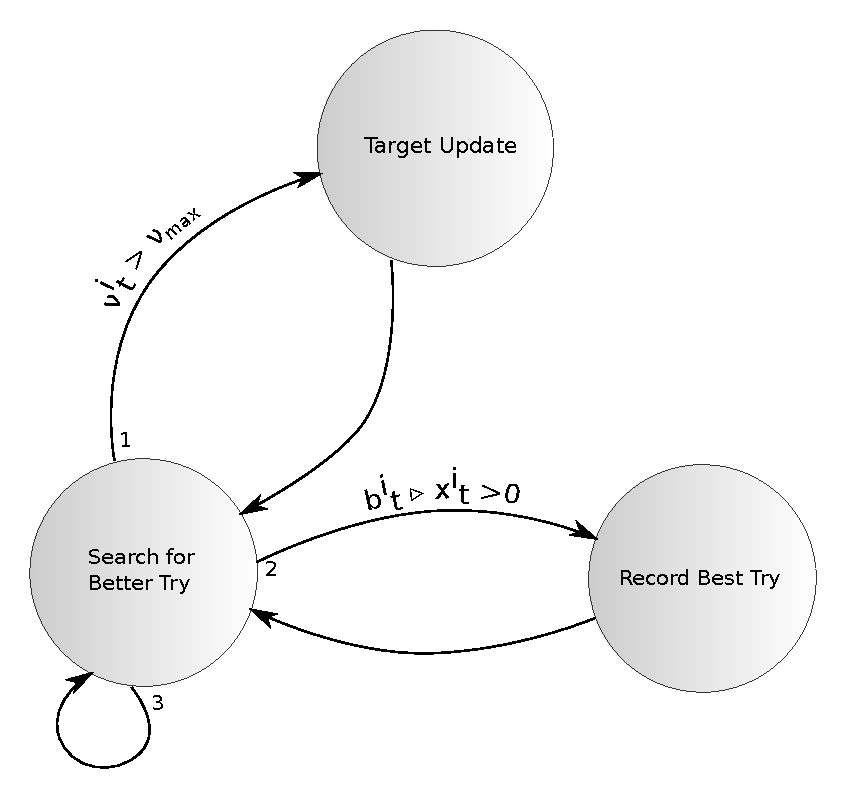
\includegraphics[width=0.7\linewidth]{CLPSO.pdf}
	\caption[CLPSO State Diagram for Determining Target]{CLPSO Target determining state diagram. The Target is only changed when the chosen target fails to give improvement in $\nu_{MAX}$ iterations.}
	\label{fig:clpso}
\end{figure}

\subsection{GPso}
GPso was the first complete SPSO coded up where all particles belong to one Group and Group target is the particle with best personal best. This  is the same choice of target as proposed for the original continuous  PSO in \cite{KE-pso}; it often gives more rapid convergence but is more easily stuck at a local minimum which is far from optimal. 

\chapter{Cost Function Factory}
\section{Cost Function interface with SPSO}
Cost function links up with a SPSO through a \emph{golang interface }called \texttt{Fun}  in \codesorc{setpso.go}. The interface is as follows: 

\begin{description}
	
	\item[NewTry() $t$ \texttt{Try}]
	creates a new Try which is a pointer to a structure  with a Try interface. A pointer is used so that as an argument in a function it can be modified by the function. As far as SPSO is concerned $t$ is opaque apart from having a Try interface to be described later. $t$ is ready to be used as a try with default Parameters  that satisfy prevailing constraints. As such a try is a container of data that matches its Parameter. 
	
	\item[SetTry($t$ \texttt{Try}, $z$ \texttt{*big.Int}) ]
	sets up  $t$ from  Parameter $z$, where $z$ is a Parameter assumed to satisfy constraints $\Omega$ and it also computes dependants such as cost etc. Note that a parameter is represented by a positive big integer and as such has the potential to have an arbitrary number of set elements.   
	
	\item[Copy($dest$, $src$ \texttt{Try})]
	sets  the $dest$ by copying $src$ to $dest$. The copy is a deep copy  and is independent of changes to $src$ once the copy is done.

	\item[UpdateCost($x$ \texttt{Try})]
	updates internal cost evaluation of a Try where a lower cost is better.
	this is needed when the cost changes or where a repeated cost evaluation is used to improve a cost estimate.  

	
	\item[Cmp($x$, $y$ \texttt{Try}, $mode$ \texttt{futil.CmpMode}) \texttt{float64}]
	 checks to see if $y$ is better than $x$ where it has the following modes:
	\begin{description}
		\item[futil.CostMode:] 	\texttt{Cmp()} compares two tries returning a value that is $x \rhd y$ with a spread of uncertainty from -1.0 to 1.0. It returns -1.0 for
		definitely $F(x) < F(y)$  and 1.0 for definitely $F(x) > F(y)$.
		A deterministic cost should always return -1.0 or 1.0 with a value of
		-1.0 if the costs are equal.
		
		\item[futil.TriesMode] (used only when cost is not deterministic)
			\texttt{Cmp()} compares how successful  $y$  has been in being better than  an $x$,
		updates $y$'s success stats leaving $x$ unchanged and returns $x \unrhd y$.
		While being compared a value $> 1.0$ indicates $y$ should replace $x$; a value
		$< -1.0$ indicates $y$ should be removed as a candidate.
	\end{description}
	
	\item[MaxLen() ($maxlen$ \texttt{int})]
	maximum number of bits in the parameter big integer which is the
	maximum number of elements in the subset.
	At the moment this is fixed during a run but in the future could vary possibly to incorporate some form of subroutine use where subroutines are added to the list of items represented by the Try Parameter.
	
	\item[About() ($s$ \texttt{string})]
	string giving a description of the cost function.
	
	\item[ToConstraint($pre$ \texttt{Try}, $hint$ \texttt{ *big.Int})\texttt{ bool}]
	this attempts to  give a constraint satisfying Try  in  $pre$ that matches the  Parameter, $hint$. 
    On success \texttt{ToConstraint()} returns \texttt{true} otherwise it returns \texttt{false} and should leave $pre$ un changed. This function enables the SPSO to pass a Try Parameter to the cost-function factory in a form of a request to update $pre$ if possible. 
    
    By convention $pre$ always is a Try (apart from when it is the default one  at the
	beginning) that was a personal best and thus satisfies the constraints required
	by the function to give a meaningful solution. The function should be able to
	find a constraint satisfying version for  $hint$ that approximates to $hint$  most
	of the time so that the SPSO can frequently change the Particle's Parameter
	during an update.
	
	\item[Delete($i$ \texttt{ int}) \texttt{bool}]
	this hints to the function to replace the $i^{th}$ particle-item.
	If it returns \texttt{True} the function has replaced the item with a new meaning
	thus modifying the decoder. 
	
\end{description}

\subsection{Catering for Changing a  Set Item}

This is an advanced feature for cost functions. Certain set items will after a
while not be used to give personal best at which point a cost function can be
hinted to remove this item through Delete() which returns \texttt{true} if the cost
function does so. if the cost function  returns true it is then up to the cost
function to either replace this by a new item with its own contribution to cost
or set the  corresponding item in a hint to zero during a successful
\texttt{ToConstraint()} call. in this way the cost function  can  try  out alternative
items that may result in an improved cost. Typically this feature is not used
and a call to  \texttt{Delete()} returns\texttt{ false}.
\section{Try Interface and Internals}
Try is data associated with a Try Parameter that comprises a copy of the parameter, internal representation of a decoded version as TryData and a cost structure for recording cost related data.
The following is the Try interface given in \codesorc{fun/futil/futil.go}:
\begin{description}
	\item[Fbits()\texttt{ float64}] returns floating point representation of cost
	as singed number of bits needed to represent cost as if an integer. This is used in plotting a cost with a logarithmic scale that works for positive and negative values returning zero if the cost is zero.
	for a continuous cost $c=F()$ we have 
	\begin{equation}\label{eqn:fbits}
		fbits(c) = \mathrm{sign}(c)\log_2(|c|+1)
	\end{equation}
    It must be remembered that, At least for the moment, Fbits() is never used by the SPSO optimiser and is only used for graphical output. 
    
    \item[Parameter() \texttt{*big.Int}]  subset parameter used by Try.
    
    \item[Decode() \texttt{string}]  this  gives a human readable interpretation of Try based on the internal decoding of the Parameter.
    
    \item[Cost() \texttt{string}] this gives human readable cost details such as variance  or mean value depending on the cost type.
    
    \item[Data() \texttt{TryData}]  decoded data part.
\end{description}

\subsection{Providing a Meaningful Interpretation of Parameters}

Representing a particle's Parameters as a binary string or subset may not be
easily  interpreted  as a meaningful representation of a solution to a
combinatorial optimization so the cost function must provide an easily
understood description of a Parameter as a string supplied by the Decode()
function.
\subsection{Try Data and its Interface}
Try Data  with interface \texttt{TryData } is used to store useful  variables value produced during decoding to  the Try Parameter and is typically only visible to the Cost Function. Try Data effectively acts as a cache so that the Parameter does not have to be decoded every time the decoded representation is used often many times while evaluating cost. For instance if the decoded Parameter is a program it is evaluated several times on test data to give a cost. The \texttt{TryData} interface has just one public method:
\begin{description}
	\item[Decode() \texttt{string}] this gives a human readable description of the data.
\end{description}
 
As will be shown in Section \ref{sec:Stubs} the main interface  that has to be coded up for each Cost Function only needs to explicitly deal with the Try Data part of a Try and choice of standard stub to represent the type of cost being used by the Cost Function thus reducing the overhead of writing one.

\section{Try Data Centric Cost Function and the Use of Stubs \label{sec:Stubs}}
the Cost Function interface given in operates at the level of Tries. Implementing this interface results in a lot of common code that only depends on the type of cost used by the Cost Function, while most of the operations specific to a Cost Function implementation involves manipulating Try Data; because of this the software supplies Cost Function stubs for each cost type that takes a Try Data manipulation cost function with the following interface in \codesorc{fun/futil/futil.go} :
\begin{description}
	\item[CreateData() \texttt{TryData}] creates an empty try data store for the decoded part of the try.
	\item[DefaultParam() \texttt{*big.Int}]  returns a default parameter which should satisfy constraints.
	\item[CopyData($ dest $,$  src $ \texttt{TryData})] copies try data from $ src  $ to $ dest $.
	\item[MaxLen() \texttt{int}] maximum number of bits used in the try parameter.
	\item[About() \texttt{string}] description of the function.
	\item[Constraint($ pre $ \texttt{TryData}, $ hint $ \texttt{*big.Int}) ($ valid $ \texttt{bool})] attempts to update $ hint $ to give a constraint satisfying try parameter possibly with the help of $ pre  $ which is assumed to be constraint satisfying. Note it is rare that $ pre $ is needed and $ pre $ should be not modified by this function.
	\item[Delete($ i  $ \texttt{int}) \texttt{bool}]  hints to the function to remove/replace the $  i^{th} $ item. Return true if the function decides to do this otherwise it returns false and does nothing.
	\item[IDecode($ data $ \texttt{ TryData},$  z $ \texttt{*big.Int})] decodes the parameter $ z $ and stores the result in $ data $.

\end{description}   
	Each Try Data manipulation cost function must have  a specific \textbf{Cost()} method for calculating a cost based on Try Data. Under the heading of each cost type  this will be referred to as the \emph{cost interface}.

\section{Standard Cost Representation Cases for a Try}
Here is a description of each cost representation.
\subsection{\texttt{SFloatFun}}
This  Try Data manipulation cost function is used when the underlying cost is  \texttt{float64} and has noise that can be removed by repeated evaluation of a cost and averaging the result with a forgetting time constant $T_c$ to allow for a slow change in cost, possibly due to a change in the environment. Time is measured as the number of iterations. The cost interface and function stub creation  are:
\begin{description}
	\item[Cost$ (data $ \texttt{TryData}) \texttt{float64}] calculates the raw cost of the try using the decoded data, returning  the cost.
	\item[NewSFloatFunStub($ f $ \texttt{SFloatFun}, $ T_c $, $ \sigma_M $ \texttt{float64}) \texttt{*SFloatFunStub} ] creates an instance of the \texttt{SFloatFunStub} ready for use as the interface \texttt{setpso.Fun}. $ T_c $ is the initial try cost update time constant; $ \sigma_M $ is a acceptance margin used in the assessment of a Tries comparison using $ \unrhd $.
\end{description}  
code is in \codesorc{fun/futil/sfloat.go}, and corresponding Try type is \texttt{SFloatTry}.

Each Try $  x $ maintains cost related variables. In the following we will refer to these variables  without referring to $x$ unless there is a need to do so. A Try has a forgetting factor $\alpha$ so if one  take measurements $ a_i, a_{i+1}, \dots $ the sum of these measurements up to $n$ using the forgetting factor is 
\begin{align}
	S_n(a) &= \sum_{k=i}^{n} a_k \alpha^{n-k} \\
	&= \alpha S_{n-1}(a)+a_n
\end{align}     
 where we take $a_{i-1}=0$. The influence from the past decays as $\alpha^{n-k}$ so the decay is exponential with time constant $T_c$ if 
 \begin{equation}\label{key}
 	\alpha^{n-k} = e^{-(n-k)/T_c}
 \end{equation}
so 
\begin{align}
	\alpha &= e^{-1/T_c}\\
			&\approxeq 1-1/T_c \label{eqn:approx-forget}
\end{align}
in the algorithm  time constant is large so we adopt the approximate version (\ref{eqn:approx-forget}) to avoid taking exponential. for notational convenience put 
\begin{align}
	S_n &= \sum_{k=i}^{n}  \alpha^{n-k} \\
	&= \alpha S_{n-1}+1
\end{align}     
then we see that if we have sequence of independent measurements of raw cost $c$ we get 
\begin{equation}\label{key}
	mean = \frac{S_n(c)}{S_n}
\end{equation}
is an unbiased estimate of the mean cost when the statistics is fixed, this is used to compare with other tries as an ongoing value for the cost $ F() $. When the Try  is initialised with a Parameter, $mean$ is set to the raw cost and uses above recursion when updated with additional raw costs. this gives an estimate of cost that improves after each update up to a point limited by the time constant $T_c$.   

For  comparison $x \rhd y$ returns 0.5 if $ F(x) > F(y)$ otherwise it returns -0.5. This indicates to SPSO that the comparison is uncertain and forces SPSO to look at $x \unrhd y$ to compare two costs. when this happens x is usually a personal best  and  the Try $y$ starts to record the success sequence $\mathbf{k}$ and the comparison sequence $\mathbf{n}$. where $\mathbf{k}_t =1$ when a comparison gives $F(x_t)>F(y_t)$ for some $x$ and is zero for other comparisons. Similarly $\mathbf{n}_t=1 $ for each such comparison. Allowing for the forgetting factor we get the frequency counts:
\begin{align}
	k_t &= S_t(\mathbf{k})\\
	n_t &= S_t(\mathbf{n})
\end{align}
This is then used to calculate an estimate of the probability that $F(x)>F(y)$  as $PT$.
\begin{equation}\label{eqn:success-estimate}
	PT_t=\frac{k_t+1}{n_t+2}
\end{equation}
this is the Bayesian estimate   with a probability prior uniformly distributed used to avoid misplacing the estimate when there is only a few measurements. $x \unrhd y$ is meant to be a score of how likely $F(x) > F(y)$  is based on $PT$. Let $\sigma_M$ be the confidence that a random sequence giving  $PT$ would be within $\sigma_M$ standard deviations of 1/2 we get using Wald's approximation such a random sequence would be within 
\begin{equation}
	PT_t \pm \sigma_M\sqrt{\frac{PT_t(1-PT_t)}{n_t}}
\end{equation}
so to ensure $y$ is better than $x$ to within $\sigma_M$ certainty we need 
\begin{equation}\label{eqn:score-threshold}
	PT_t-\sigma_M \sqrt{\frac{PT_t(1-PT_t)}{n_t}} >1/2
\end{equation}
this is equivalent to 
\begin{align}
	s_t&= \frac{n_t r_t}{\sigma^2_M }>1 \, \wedge PT_t> 1/2\\
	r_t&= \frac{(PT_t-1/2)^2}{PT_t(1-PT_t)} 
\end{align}
this in turn is equivalent to
\begin{align}
	\epsilon_t &= PT_t-1/2 \\
	r_t &=\frac{ \epsilon^2_t}{1/4 - \epsilon^2_t} \\
	s_t&=\frac{n_t r_t}{\sigma^2_M }>1 \, \wedge \epsilon_t > 0
\end{align} 
from this we get an appropriate score
\begin{equation}\label{eqn:candidate-score}
	x \unrhd y = \left\lbrace 
	\begin{array}{cc}
		s_t &\mathrm{ if}\; \epsilon_t >0\\
		-s_t& \mathrm{otherwise}
	\end{array}\right .
\end{equation}
which is used by the algorithm to give a  credentials score.      

\subsection{\texttt{FloatFun}}
This  Try Data manipulation cost function is used when the underlying cost is  \texttt{float64} and the computed cost is a deterministic function of the Try Parameter. The cost interface and function stub creation  are:
\begin{description}
	\item[Cost$ (data $ \texttt{TryData}) \texttt{float64}] calculates the raw cost of the try using the decoded data, returning  the cost as $F()$.
	\item[NewFloatFunStub($ f $ \texttt{FloatFun}) \texttt{*FloatFunStub} ] creates an instance of the \texttt{FloatFunStub} ready for use as the interface \texttt{setpso.Fun}. 
\end{description}  
code is in \codesorc{fun/futil/float.go}, and corresponding Try type is \texttt{FloatTry}.

\subsection{\texttt{IntFun}}
This  Try Data manipulation cost function is used when the underlying cost is  \texttt{*big.Int} and the computed cost is a deterministic function of the Try Parameter. The cost interface and function stub creation  are:
\begin{description}
	\item[Cost$ (data $ \texttt{TryData}, cost \texttt{*big.Int})] calculates the raw cost of the try using the decoded data, returning  the result in cost as $F()$.
	\item[NewIntFunStub($ f $ \texttt{IntFun}) \texttt{*IntFunStub} ] creates an instance of the \texttt{IntFunStub} ready for use as the interface \texttt{setpso.Fun}. 
\end{description}  
code is in \codesorc{fun/futil/int.go}, and corresponding Try type is \texttt{IntTry}.
\subsubsection{Using Big Integer}
Big integer cost values are used to include some of the difficult cases in combinatorial optimisation, although the chance of finding global best solutions to these problems is minimal; however, The algorithms are expected to produce good useful approximations to these hard problems; I would like to suggest that main area of application is \emph{machine learning where one is interested in good approximate minimisation solutions of difficult problems}.







\part{Miscellaneous Ideas}
\chapter{Statistics}


\section{Recursive formula for calculating expected values}


Let $S$ be a finite set and $P:2^S \longrightarrow [0,1]$ be the probability of subsets of $S$
Let $b_{i}$ be a sequence of independent samples of subsets of $S$ 
representing $P$. 

For a subset $A\subset S$ and a map $g:2^{A}\rightarrow\mathbb{R}$
we can get a sequence of estimates of expected values
\[
\mathbb{E}_{n}[g\parallel A]=\frac{1}{n}\sum_{i=1}^{n}g(b_{i}\cap A)
\]
of 
\[
\mathbb{E}[g\parallel A]=\sum_{B\subset S}P(B)g(B\cap A)
\]
which just calculates the expected value of $g$ acting on subsets
of $A$ . The double bar notation $\parallel$ is used to indicate
that we are looking on to the probability distribution through the
sub set window $A$. Now for $n>1$ 
\[
\mathbb{E}_{n}[g\parallel A]=\left(1-\frac{1}{n}\right)\mathbb{E}_{n-1}[g\mid A]+\frac{1}{n}g(b_{n}\cap A)
\]
we can generalise this to the sequence 
\[
\check{\mathbb{E}}_{n}[g\parallel A]=\left(1-\lambda_{n}\right)\mathbb{\check{E}}_{n-1}[g\parallel A]+\lambda_{n}g(b_{n}\cap A)
\]
with 
\[
\check{\mathbb{E}}_{1}[g\parallel A]=g(b_{1}\cap A)
\]
taking expected values and putting $\mathbb{\tilde{E}}_{n}[g\parallel A]=\mathbb{E}\left[\check{\mathbb{E}}_{n}[g\parallel A]\right]$
we get
\begin{align}
\mathbb{\tilde{E}}_{n}[g\parallel A] & = (1-\lambda_{n})\mathbb{\tilde{E}}_{n-1}[g\parallel A]+\lambda_{n}\mathbb{E}[g\parallel A]\\
& = (1-\lambda_{n})\mathbb{\mathbb{E}}[g\parallel A]+\lambda_{n}\mathbb{E}[g\parallel A]\\
& = \mathbb{E}[g\parallel A]
\end{align}

by induction on $n$. So even this sequence is an unbiased estimate
of the expected value. The important thing is to check for variance.
We have
\begin{align*}
\mathbb{E}\left[\left(\mathbb{\check{E}}_{n}[g\parallel A]-\mathbb{E}[g\parallel A]\right)^{2}\right] & = \mathbb{E}\left[\left(\mathbb{\check{E}}_{n}[g\parallel A]\right)^{2}\right]-2\mathbb{E}\left[\mathbb{\check{E}}_{n}[g\parallel A]\right]\mathbb{E}[g\parallel A]+\mathbb{E}[g\parallel A]^{2}\\
& = \mathbb{E}\left[\left(\mathbb{\check{E}}_{n}[g\parallel A]\right)^{2}\right]-\mathbb{E}[g\parallel A]^{2}\\
& = (1-\lambda_{n})^{2}\mathbb{E}\left[\left(\mathbb{\check{E}}_{n-1}[g\parallel A]\right)^{2}\right]+\lambda_{n}^{2}\mathbb{E}\left[g(b_{n}\cap A)^{2}\right]+(2\lambda_{n}(1-\lambda_{n})-1)\mathbb{E}[g\parallel A]^{2}\\
& = (1-\lambda_{n})^{2}\mathbb{E}\left[\left(\mathbb{\check{E}}_{n-1}[g\parallel A]\right)^{2}\right]+\lambda_{n}^{2}\mathbb{E}\left[g(b_{n}\cap A)^{2}\right]-((1-\lambda_{n})^{2}+\lambda_{n}^{2})\mathbb{E}[g\parallel A]^{2}\\
& = (1-\lambda_{n})^{2}\mathbb{E}\left[\left(\mathbb{\check{E}}_{n-1}[g\parallel A]-\mathbb{E}[g\parallel A]\right)^{2}\right]+\lambda_{n}^{2}\mathbb{E}\left[\left(g(b_{n}\cap A)-\mathbb{E}[g\parallel A]\right)^{2}\right]
\end{align*}
where we have used the independence of the $b_{i}$'s to give
\begin{align*}
\mathbb{E}\left[\mathbb{\check{E}}_{n-1}[g\parallel A]g(b_{n}\cap A)\right] & = \mathbb{E}\left[\check{\mathbb{E}}_{n-1}[g\parallel A]\right]E\left[g(b_{n}\cap A)\right]\\
& = \mathbb{E}[g\parallel A]^{2}
\end{align*}
put
\begin{align*}
\sigma^{2} & = \mathbb{E}\left[\left(g(b_{n}\cap A)-\mathbb{E}[g\parallel A]\right)^{2}\right]\\
\alpha_{n} & = \nicefrac{\mathbb{E}\left[\left(\mathbb{\check{E}}_{n}[g\parallel A]-\mathbb{E}[g\parallel A]\right)^{2}\right]}{\sigma^{2}}
\end{align*}
then we have
\[
\alpha_{n}=(1-\lambda_{n})^{2}\alpha_{n-1}+\lambda_{n}^{2}
\]
as a formulae that gives the change in variance of the estimates $\check{\mathbb{E}}_{n}[g\parallel A]$
.

As one can see there are several ways of combining measured means to give unbiased estimates of a noisy function's mean that gives a trade off on variance.
 


To directly calculate the expected cost at each iteration would be too expensive an operation especially if the parameters are way off optimal. Let $C(X)$ be the random variable representing the cost function for a given parameter vector $X$. for a given particle the current parameter changes rapidly while when it matters the personal best parameter, $X_b$ varies comparatively slowly so  when the $X_b$ is not updated one can take the opportunity to update the estimated expected cost function value $\hat{C}(X_b)$ of $\mathbb{E}[C(X_b)]$ in this case.This reduces the variance of the expected value compared to its raw value $C(X_b)$. 

Lets look at some ways in which the estimate in principle can be updated iteratively. Given samples $C_1,\cdots,C_i$ and a forgetting gain $\alpha$ we could produce an unbiased estimate
\begin{equation}
\label{est1}
\hat{C}(X_b)_i=\frac{\sum_{j=1}^i\alpha^{j-1}C_{i-j+1}}{\sum_{j=1}^i\alpha^{j-1}}
\end{equation}
Put 
\begin{align}
A_i&=\sum_{j=1}^i\alpha^{j-1}\\
\label{sum_a}
&=\frac{1-\alpha^i}{1-\alpha}
\end{align}
then using \eqref{est1} we get
\begin{align}
A_{i}\hat{C}(X_b)_{i}-\alpha A_{i-1}\hat{C}(X_b)_{i-1}=C_i
\end{align}
rearranging and using \eqref{sum_a} we get
\begin{align}
\hat{C}(X_b)_{i}&=\frac{\alpha A_{i-1}\hat{C}(X_b)_{i-1}+C_i}{A_{i}}\\
\label{est2}
&=\frac{\alpha(1-\alpha^{i-1})\hat{C}(X_b)_{i-1}+(1-\alpha)C_i}
{1-\alpha^{i}}
\end{align}
now if we put 
\begin{equation}\label{lam1}
\lambda_i=\frac{1-\alpha}{1-\alpha^{i}}
\end{equation}
we get substituting into \eqref{est2} the iterative update
\begin{equation}\label{est3}
\hat{C}(X_b)_{i}=(1-\lambda_i)\hat{C}(X_b)_{i-1}+\lambda_i C_i
\end{equation}
In fact any update of the form given in \eqref{est3} always gives an unbiased estimate  for arbitrary $\lambda_i$ . So we can use this as a generalised update. the choice of parameter is tuned to cater for how rapidly one wants to converge and the required variance of the result.

Looking at the variance update assuming independent samples. Put $\sigma_i^2$ as the variance of $\hat{C}(X_b)_{i}$ and $\sigma^2$ as the variance of $C_i$ then we get
\begin{equation}\label{vari1}
\sigma_i^2=(1-\lambda_i)^2\sigma_{i-1}^2 +\lambda_i^2 \sigma^2
\end{equation} 
The minimum value of the update variance as a function of $\lambda_i$ occurs at the point of inflexion given by
\begin{align}
0=&\frac{\partial \sigma_i^2}{\partial \lambda_i}\\
=&-2(1-\lambda_i)\sigma_{i-1}^2+2\lambda_i \sigma\\
=&2\{ \lambda_i(\sigma_{i-1}^2 + \sigma^2) -\sigma_{i-1}^2\}
\end{align} 
This gives the smallest variance $\lambda_i$ as
\begin{align}
\stackrel{*}{\lambda_i} &= \frac{\sigma^2}{\sigma_{i-1}^2 + \sigma^2}\\
&=\frac{1}{1+(\frac{\sigma^2}{\sigma_{i-1}^2})} \label{lam_st1}\\
&=\frac{\sigma^{-2}}{\sigma_{i-1}^{-2} + \sigma^{-2}}
\label{lam_st2}
\end{align}
From \eqref{lam_st2} we get
\begin{equation}\label{lam_st3}
1-\stackrel{*}{\lambda_i} =\frac{\sigma_{i-1}^{-2}}{\sigma_{i-1}^{-2} + \sigma^{-2}} 
\end{equation}
\eqref{lam_st1} show that the result depends only on the ratio of variances while \eqref{lam_st2} gives the result in form of inverse variance. using this gives easy to use results as will shortly be seen. Based in this remark substitute \eqref{lam_st2},\eqref{lam_st3} into \eqref{vari1} and calculate the updated inverse variance as
\begin{align}
\stackrel{*}{\sigma_i}^{-2}&=((1-\stackrel{*}{\lambda_i})^2\sigma_{i-1}^2 +\stackrel{*}{\lambda_i}^2 \sigma^{2})^{-1}\\
&=\frac{\sigma_{i-1}^{-2} \sigma^{-2}}{(1-\stackrel{*}{\lambda_i})^2\sigma^{-2} +\stackrel{*}{\lambda_i}^2 \sigma_{i-1}^{-2}}\\
&=\frac{\sigma_{i-1}^{-2}\sigma^{-2}(\sigma_{i-1}^{-2} + \sigma^{-2})^2 }{\sigma_{i-1}^{-4}\sigma^{-2} + \sigma_{i-1}^{-2}\sigma^{-4}}\\
&=\sigma_{i-1}^{-2}+\sigma^{-2} \label{inv_var1}
\end{align}  
This shows the inverse variance using the optimal $\lambda$ is additive and the expression is particularly simple so it can be calculated first and then $\stackrel{*}{\lambda_i}$ is evaluated from
\begin{equation}\label{lam_st4}
\stackrel{*}{\lambda_i}=\sigma^{-2}/\stackrel{*}{\sigma_{i}}^{-2}
\end{equation} 
This gives the minimum variance update. However in the long run as it repeats the $\lambda_i$ becomes so small that it ignores the current measurement and any change in the underlying statistics is ignored. We can avoid this by deliberately choosing a $\lambda_i$ which is larger than the optimal given by \eqref{lam_st4}. To this end put 
\begin{equation}\label{nlam1}
\lambda_i = (1+\delta)\stackrel{*}{\lambda_i}
\end{equation} 
then evaluate the updated inverse variance by substituting into
\eqref{vari1} the expression \eqref{nlam1} and simplifying using \eqref{inv_var1},\eqref{lam_st2} and \eqref{lam_st3}
\begin{align}
\sigma_i^{-2}&= \frac{\sigma^{-2} \sigma_{i-1}^{-2}}
{[(1-\stackrel{*}{\lambda_i})-\delta \stackrel{*}{\lambda_i}]^2\: \sigma^{-2}+\stackrel{*}{\lambda_i}^2 (1+\delta)^2\: \sigma_{i-1}^{-2}}\\
&= \frac{\sigma^{-2} \sigma_{i-1}^{-2}}{(1-\stackrel{*}{\lambda_i})^2\:\sigma^{-2}+ \stackrel{*}{\lambda_i}^2\:\sigma_{i-1}^{-2} 
	-2(1-\stackrel{*}{\lambda_i})\:\sigma^{-2}
	+2\stackrel{*}{\lambda_i}\sigma_{i-1}^{-2}
	+\stackrel{*}{\lambda_i}^2\delta^2(\sigma^{-2}+\sigma_{i-1}^{-2}) }	\\
&=\frac{\sigma^{-2}\sigma_{i-1}^{-2}\stackrel{*}{\sigma_i}^{-4} } 
{\sigma^{-2}\sigma_{i-1}^{-2}\stackrel{*}{\sigma_i}^{-2}+\sigma^-4 \stackrel{*}{\sigma_i}^{-2}\delta^2 }\\
&=\frac{\stackrel{*}{\sigma_i}^{-2}}
{1+\sigma^{-2}/\sigma_{i-1}^{-2}\:\delta^2 }\label{nlam2}
\end{align}

Equation \eqref{nlam2} is a particularly simple expression that shows how the inverse variance depends on $\delta$.


Most models of probability distribution start with combining pairs
of variables to give more elaborate models of the probability function.
Often in the case of neural nets the pairs are combined linearly
to give a single linear function which is then threshold before
being passed onto an output or hidden layer. Unfortunately this in
the case of neural nets gives rise to difficult to interpret models
with with often pathological behaviour. The aim here is to use the
multilinear approach that encourages more unique representation of
the data which can also be interpreted. However multi-linear functions
are only linear on each variable in isolation and are in general non
linear, hopefully in a useful way. When combining pairs of variables
we will combine to produce a result for a hidden variable (or output
from this ) and not threshold it. This section gives
results for combining pairs of variables. 
\section{Cost-function Value Representation} \label{Sec:CostValue} 
Here is a cost function value representation that has been superseded but contains an interesting iterative method for calculating mean and variance subject to including a history forgetting process. The code for it is at 

\codesorc{fun/futil/s0float.go}.
\subsection{\texttt{S0FloatCostValue} implementaation of \texttt{CostValue}}

In the targeted application of Machine Learning the cost-function  value $F(x)$ is not a direct mathematical function of $x$ and has a random component so it has to be evaluated several times before comparing the fitness of $x$. \texttt{S0FloatCostValue}  was used in this case if the underlying mean value is the cost to minimise.  Even if the  cost function is deterministic, The evaluation of a cost value may include a very large number of tests to evaluate  the cost. for instance the cost may be a measure of a program output miss match for all possible inputs. faced with this a small set of randomly selected test cases is used instead. Each time there is a need to calculate another value a fresh set of random samples is used to generate another approximate cost. To keep things simple assume that each cost sample is independent for a given $x$ and that the statistics of $F(x)$ for a given $x$ is slowly varying with a time constant of at least $T_C$. The idea is that  \texttt{S0FloatCostValue}  maintains a mean and variance running value subject to the time constant constraint. 

Let $x,y $   be two parameters  for comparison that has the corresponding estimated mean $C_x,C_y $and estimated  variance $\sigma^2C_x, \sigma^2C_y$ of these respective means .  The noisy raw cost signal is replaced by the mean estimates for comparison. Put
\[ \Delta=(C_x-C_y)^2 -(\sigma_{thres})^2(\sigma^2C_x+\sigma^2C_y) \]
the difference is regarded as significant if 
\[  \Delta>0\]
for some comparison threshold $\sigma_{thres} $ used as a heuristic.\footnote{ normally $ \sigma_{thres}$ is independent of the cost value but in the code is stored by $F(x)$; in the code $x,y$ is used as in $F(x).Cmp(F(y) $ so there is a slight lack of symmetry in the treatment of $(x,y)$  } As more measurements are included the variance of estimates reduces. As will be shown the time constant constraint stops this variance reduction beyond a certain point at which  the  variance is time constant limited. We get the following cases:
\begin{list}{}
	\item $F(x)<F(y)$  when $\Delta >0$ and $C_x<C_y$
	\item $F(x)>F(y)$  when $\Delta >0$ and $C_x>C_y$	
	\item $F(x) \leftthreetimes F(y)$  when $\Delta \le 0$  and $\sigma ^2C_x>sigma^2C_y$ with $\sigma ^2C_x,\sigma ^2C_y$ not time constant limited.
	\item $F(x) \leftthreetimes F(y)$  when $\Delta \le 0$  and $\sigma ^2C_y$ is time constant limited but $\sigma ^2C_x$ is not.
	\item $F(x) \rightthreetimes F(y)$   when $\Delta \le 0$  and $\sigma ^2C_x \le \sigma^2C_y$ with $\sigma ^2C_x,\sigma ^2C_y$ not time constant limited.
	\item $F(x) \rightthreetimes F(y)$ when $\Delta \le 0$  and $\sigma ^2C_x$ is time constant limited but $\sigma ^2C_y$ is not.
	\item $F(x)=F(y)$    for all other cases.			
\end{list} 
The idea is to carry on asking for cost function updates until the difference in the estimated means are significant, always asking for further evaluations that are likely to achieve this and failing this regard the  cost values to be effectively equal. 

\subsubsection{ evaluating running mean and its variance}
This leads to how the $C$ and $\sigma ^2C$ are evaluated. Let $(x_0, \ldots, x_ j \dots )$ be a sequence of raw cost values produced by the cost function for a  parameter $x$ then intuitively an estimate of the mean $C_j$ minimises
\begin{equation}\label{eq:J_j}
J_j=\frac{1}{2}\sum_{i=0}^{i=j}\alpha_{j\:i}(x_i-C_j)^2
\end{equation}
where the $\alpha_{j\:i}$ are chosen to be of the form 
\begin{equation}\label{eq:alpha_def}
\alpha_{j\:i}=\prod_{k=i+1}^{j}b_k\: \mathrm{for}\: j>i ;\; \alpha_{j\:j}=1
\end{equation}
The $b_k$ can be regarded as forgetting weights and for the moment has a value between 0 and 1. the form of $\alpha_{j\:i}$  has been chosen to give incremental updates. Choose $C_j$ to minimise $J_j$ so the derivative with respect to $C_j$ will be zero giving
\begin{equation}\label{eq:J_zero_diff}
0=\dfrac{\partial J_j}{\partial C_j} =-\sum_{i=0}^j (x_i-C_j)\alpha_{j\:i}
\end{equation}
which gives
\begin{equation}\label{eq:C_j_def}
C_j= D_j \lambda_j
\end{equation}
where
\begin{align}
D_j =&\sum_{i=0}^j x_i \alpha_{j\:i}\label{eq:D_j_def} \\
\lambda_j=\beta_j^{-1};\:\beta_j=&\sum_{i=0}^j \alpha_{j\:i}\label{ eq:lambda_j_def}
\end{align}
Later on we will need
\begin{align}\label{delta_j_def}
\delta_j=&\sum_{i=0}^j \alpha_{j\:i}^2\\
I_j=&\lambda_j \sum_{i=0}^j \alpha_{j\:i} x_i^2
\end{align} 
using \ref{eq:alpha_def} we get the following iterative evaluations for $j > i\geq 0$
\begin{align}
\alpha_{j\:i}=&b_j \alpha_{j-1\:i}\\
\beta_j=&b_j \beta_{j-1} + 1;\:\beta_0=1 \label{eq:beta_j_iter}\\
\lambda_j=&\frac{\lambda_{j-1}}{\lambda_{j-1} + b_j} ; \: \lambda_0=1  \label{eq:lambda_iter}\\
D_j=&b_j D_{j-1} + x_j ; \: D_0=x_0\\
\delta_j=& b_j^2 \delta_{j-1}+1 \label{eq:delta_iter}
\end{align}
from this we get an iteration rule for $C_j$
\begin{align}
C_j=&(b_j D_{j-1} + x_j)\lambda_j \\
=& \frac{b_j D_{j-1} \lambda_j}{\lambda_j +b_j} +x_j \lambda_j \\
=&(1-\lambda_j)C_{j-1} + x_j \lambda_j : \: C_0=x_0 \label{eq:c_j_iter}
\end{align}
Similarly we get the iteration
\begin{align}
I_j=& (1-\lambda_j)I_{j-1}+\lambda_j x_j^2; \: I_0=x_0^2
\end{align}
To get a handle on the statistics assume that it is effectively constant with the samples of $x_j$ being independent with mean $\mu$ and variance $\sigma^2 $ then taking expected values we get
\begin{align}
\mathbb{E}(C_j)=& (1-\lambda_j)\mathbb{E}(C_{j-1})+\mathbb{E}(x_j)\lambda_j\\
=& (1-\lambda_j)\mu +\lambda_j \mu\\
=&\mu
\end{align}
by induction, so $C_j$ is an unbiased estimate of the mean as expected. 
To calculate the variance of $C_j$ first calculate
\begin{align}
\mathbb{E}(C_j^2)=& \lambda_j ^2  \mathbb{E}\{ (\sum_{i=0}^{j} x_i \alpha_{j\:i} )  (\sum_{k=0}^{j} x_k \alpha_{j\:k} )\}\\
=&\lambda_j ^2  \{\sum_{i=0}^j \mathbb{E}(x_i^2)\alpha_{j\:i}+\sum_{i \ne k} \mathbb{E}(x_i)\alpha_{j\:i}\mathbb{E}(x_k)\alpha_{j\:k}\}\\
=&\lambda_j ^2  \{  (\sigma^2+\mu^2)\delta_j +\mu^2 \beta_j^2 -\mu^2 \delta_j  \}\\
=&\sigma^2 \delta_j  \lambda_j ^2 + \mu^2
\end{align}
so the variance of $C_j$ is given by
\begin{equation}\label{eq:C_j_variance}
\sigma^2 C_j = \sigma^2 \delta_j  \lambda_j ^2 
\end{equation}
Now
\begin{align}
\mathbb{E}(I_j)=&\lambda_j \sum_{i=0}^j \alpha_{j\:i} \mathbb{E}()x_i^2)\\
=&\lambda_j \beta_j (\sigma^2 +\mu^2)\\
=& \sigma^2 +\mu^2
\end{align}
from this we get for
\begin{align}\label{key}
\gamma_j=& \frac{\delta_j \lambda_j^2}{1-\delta_j \lambda_j^2}\\
K_j =& \gamma_j(I_j-C_j^2)\\
\mathbb{E}(K_j)=&\gamma_j \{ \mathbb{E}(I_j)- \mathbb{E}(C_j^2)  \} \\
=& \gamma_j \{ \sigma^2 +\mu^2 -  \sigma^2 \delta_j  \lambda_j ^2 -\mu^2  \}\\
=&  \frac{\delta_j \lambda_j^2}{1-\delta_j \lambda_j^2} (1-\delta_j \lambda_j^2)\sigma^2\\
=&  \sigma^2 \delta_j  \lambda_j ^2 
\end{align}
so  $K_j$ is an unbiased estimate of $ \sigma^2 C_j  $, so we can use $C_j$ as the running estimate of  mean and $K_j$ as  estimate of $C_j$ variance.
\subsubsection{choosing values for $b_j$}
All that remains is to choose  the $b_j$ which is limited to be in the range $[0, 1]$.  by Equations \ref{eq:C_j_variance}, \ref{eq:delta_iter}, \ref{eq:delta_iter} we can see that 
\begin{align}
\frac{\partial \sigma^2 C_j}{\partial b_j}=& \frac{\partial}{\partial b_j} \left[\sigma^2\frac{\lambda_{j-1}^2(b_j^2 \delta_{j-1}+1) }{(\lambda_{j-1}+b_j )^2} \right]\\
=&-2\sigma^2\lambda_{j-1}^2\frac{\delta_j b_j^2 +1  -b_j \delta_{j-1}(\lambda_{j-1}+b_j)}{(\lambda_{j-1} + b_j)^3} \\
=& -2\sigma^2\lambda_{j-1}^2\frac{(1  -b_j \delta_{j-1}\lambda_{j-1})}{(\lambda_{j-1} + b_j)^3} \label{ eq:C_var_b_slope   } \\
\end{align}
Now by using the restricted range for $b_j$ and Equations \ref{ eq:lambda_j_def}, \ref{eq:beta_j_iter}, \ref{eq:beta_j_iter} and the fact that $b_j^2\le b_j$ we get by induction that
\begin{equation}
0 \le b_j \lambda_j \delta_j \le 1
\end{equation}
so pluging this into Equation \ref{ eq:C_var_b_slope   } gives 
\begin{equation}
\frac{\partial \sigma^2 C_j}{\partial b_j} \le 0
\end{equation}
so the largest $b_j$ gives the best decrease in the variance of  $C_j$. also if we put $b_j = 0$ we get no change in the variance  from the previous variance so we also have
\begin{equation}
sigma^2 C_j\le sigma^2 C_{j-1}
\end{equation}
as well as this we get a decrease in $\lambda_j$ at each stage. However, if  $\lambda_j$ gets too small  the estimates start to ignore any changes in the statistics so we need to restrict $\lambda_j$ to ensure it has a time constant of not more than $T_C $ this means that
\begin{align}
1-\lambda_j \le e^{-1/T_C}
\end{align}  
since  the time constant is large we can use the approximation 
\begin{equation}
\lambda_j \ge 1/T_C
\end{equation}
So to get the best reduction of  $\sigma^2 C_j$ we keep $b_j = 1$ until  $\lambda_j$ hits the time constant limit and set
\begin{align}
\lambda_j =& 1/T_C \\
b_j =& 1-\lambda_j
\end{align}
to stop any further increase in the time constant of the iterative update.


\section{Multi-linear functions and binary data probabilities}

Multi-linear expressions are a natural way of generating functions of
binary data. Let $S$ be a finite ordered set of size $n$ containing
the elements $x_{1},x_{2},\cdots,x_{n}$ then we can for each binary
sequence $a:S\rightarrow\{0,1\}$ of $n$ $0$ and $1$'s associate
a subset $\varphi(a)\subset S$ given as the elements $x_{i}$ of
$S$ such that the sequence $a$ maps $a(i)$ to $1$. Put for $A\subset S$
\[
Q(A)[x_{1},x_{2},\cdots,x_{n}]=\prod_{x_{i\in A}}x_{i}\prod_{x_{j}\notin A}(1-x_{j})
\]
Let $A,B\subset S$ such that $A\neq B$ then there exists an $k$
such that either $x_{k}\in A$ and $x_{k}\notin B$ or $x_{k}\in B$
and $x_{k}\notin A$ . assuming the former and let b be the associated
binary sequence of $B$. Evaluating $Q(A)$ with b we get that $b(k)=0$
so 
\[
Q(A)(b)\triangleq Q(A)(b(1),b(2),\ldots,b(n))=\prod_{x_{i\in A}}b(i)\prod_{x_{j}\notin A}(1-b(j))=0
\]
similarly for the other case. Also $Q(B)(b)=1$ by inspection. This
also shows that the $Q(A)[x_{1},x_{2},\cdots,x_{n}]$ are linearly
independent since if
\[
\sum_{A\subset S}c(A)Q(A)[x_{1},x_{2},\cdots,x_{n}]=0
\]
for coefficients $c(A)\in\mathbb{R}$ by substituting $a=\varphi^{-1}(A)$
we get
\[
c(A)=c(A)Q(A)(a)=0
\]
If we put for $A\subset S$
\[
\widetilde{Q}(A)[x_{1},x_{2},\cdots,x_{n}]=\prod_{x_{i\in A}}x_{i}
\]
then by induction on $n$ we can show that $Q(A)$ is a linear combination
of $\widetilde{Q}(A)$. Also by definition the $\widetilde{Q}(A)$
are independent and have the same number of dimensions $2^{n}$ so
span the same subspace of polynomials. Because of this the $Q(A)$
for $A\subset S$ span the space of \emph{multilinear polynomials}.

Further for each map $f:\,2^{S}\rightarrow\mathbb{R}$ we can associate
a a polynomial $Q(f)$ over the elements of $S$ given by
\[
Q(f)[x_{1},x_{2},\cdots,x_{n}]=\sum_{A\subset S}f(A)Q(A)
\]
and we get 
\[
Q(f)(b)=f(\varphi(b))
\]
This multi-linear or polynomial representation of the map $f$ is
in one to one correspondence so there is nothing added by using the
more complex polynomial representation of the map from subsets of
$S$ other than providing a smooth continuous representation of such
functions that can be easily approximated by simple combination of
polynomials that can be used to provide a more compact approximation
of $f$. In the general case $Q(f)$ is a large expression to evaluate
or store in a computer since it has $2^{n}$ terms. Also the coefficients
by themselves do not convey any useful structure or pattern without
further analysis. The question is can one introduce more restrictive
polynomial expressions that approximate $Q(f)$ and give easy interpretations
of the underlying patterns of sequences that generate significant
values of $f$ without significant loss of information.

In particular if $P(a)$ is the probability of the sequence $a$ then
$Q(P\circ\varphi^{-1})$ is a polynomial that maps binary sequences
to their respective probability. Call this the \emph{probability polynomial}
and Use the notation $Q_{P}[x_{1},x_{2},\cdots,x_{n}]$ for this.
The $\varphi$ map is an equivalence between subsets and binary sequences
so when not ambiguous leave it out. For instance $P(A)\triangleq P(\varphi^{-1}(A))$
for a subset $A$.

As a general rule low order polynomial representations avoid over
fitting so polynomials involving a small number of variables ( that
is elements of $S$ ) are useful. in particular combining variables
in pairs is useful especially if we create intermediate variables
called hidden  that represent linear polynomials of variables
and hidden variables. 
\subsection{bivariate binary table polynomial representation}
let $x$ and $y$ be binary valued variables. let $a:\{0,1\}\times\{0,1\}\rightarrow\{0,1\}$ be a function. this is  represented by a polynomial
\begin{align}
Q(a)[x,y]=&a(0,0)(1-x)(1-y)+a(0,1)(1-x)y + a(1,0)x(1-y)+a(1,1)xy \\
=&a(00)+[a(1,0)-a(0,0)]x+[a(0,1)-a(0,0)]y+[a(0,0)+a(1,1)-a(0.1)-a(1,0)]xy
\end{align} 
that agrees with the binary function $a$ for binary values. we can get a clean uncluttered parametrisation by putting
\begin{align}
X_0&=a(0,0)\\
X_1&=a(1,0)-a(0,0)\\
X_2&=a(0,1)-a(0,0)\\
x_3&=a(1,1)-a(0,0)\\
\end{align}   
to give 
\begin{equation}
\label{bin1}
Q(a)[x,y]=X_0+X_1x+X_2y+(X_3-X_1-X_2)xy
\end{equation}

\chapter{Parking Place}
This provides a place to put text snippets while rearranging the document.




\bibliographystyle{alpha}
\bibliography{AiPlayC.bib}



\end{document}